\section{Timeline}

\subsection{Initial project meetings}

\begin{itemize}
	\item we decided to initially structure the project into
		\begin{itemize}
			\item core translation memory
			\item userspace
			\item graphical user interface
		\end{itemize}
	\item we assigned project members to specific project modules
	\item we discussed ways of acquiring initial data to fill the translation memory
		\begin{itemize}
			\item existing subtitle corpora (e.g.\ at UFAL)
			\item general purpose corpora
			\item subtitle database websites (e.g.\ \url{www.opensubtitles.org})
		\end{itemize}
	\item we discussed possible database systems to be used in the implementation
\end{itemize}


\noindent\textbf{Discussion of the decisions}
\begin{itemize}
	\item Although we added further modules, we consistently kept the initial project separation into \emph{Core}, \emph{Userspace} and \emph{GUI}. Initially, the scripts for preparing the initial data were written in Perl and classes to import the data were in the \emph{Core} module. However, to be more consistent, we decided to move the data preparation and data import to a separate \emph{dataimport} module and re-wrote the Perl scripts in Scala.
\end{itemize}

\subsection{Early implementation decisions}

\begin{itemize}
	\item We decided to base the project on the \emph{Java Virtual Machine}. Most parts should be written in Java and some parts would be written in the Scala programming language.
	\item For dependency management, we decided to use Apache Maven.
\end{itemize}

\noindent\textbf{Discussion of the decisions}

\begin{itemize}
	\item We are generally satisfied with the decision to base the project on the JVM since both the usage of Google Web Toolkit and other modules, as well as the possibility to combine all parts of the project with Apache Maven were helpful. 
	
	The decision to use both Java and Scala showed to be a difficult decision. On the one hand, Scala allowed to write concise and efficient code, on the other hand most project members were not able to learn Scala sufficiently and hence used only Java. Although the interoperability between Scala and Java works well in most cases because both are based on the JVM, some problems remain. One of the problems of interoperability was, for example, that the implementation of the datatype \emph{List} that was created in Scala was not compatible with Google Web Toolkit, which expected a standard Java \emph{List} implementation.
\end{itemize}

\begin{figure}[h]
\begin{center}
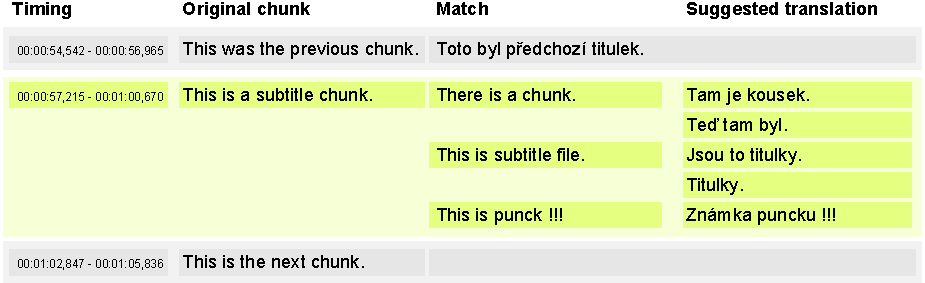
\includegraphics{./figures/original_strucutre.pdf}
\end{center}

\caption{Scheme of the originally intended structure of work with the translation memory. Reflects the original User Space structure and also schematically the original client design.}

\end{figure}


\subsection{Acquiring parallel data}

\begin{itemize}
	\item TODO
\end{itemize}


\subsection{Database evaluations and choice of GUI framework}

\begin{itemize}
	\item We evaluated different DBMS and decided to use Postgres (see section~\ref{sec:dbms}).
	\item We decided to use Google Web Toolkit for the GUI.

\end{itemize}


\subsection{Agreement on shared classes}

\begin{itemize}
	\item We agreed on the shared classes that all parts of the project should use. For best compatibility between  \emph{Core}, \emph{Userspace} and the GWT-based \emph{GUI}, we decided to write all shared classes in Java.
\end{itemize}


\noindent\textbf{Discussion of the decision}

\begin{itemize}
	\item It showed to be an important decision to agree on the shared classes early in the project since it made the cooperation between the modules easier and less verbose.
\end{itemize}


\subsection{Core design decisions}



\subsection{Userspace design decisions}



\subsection{GUI design decisions}




